% This is a default-selection of plugins that are used widely in this repo.

\documentclass[a4paper,10pt,fleqn]{article}
\usepackage[utf8]{inputenc}

% deutsche Trennmuster etc.
\usepackage[ngerman]{babel}
\usepackage[T1]{fontenc}

% mathematical simbols and fonts
\usepackage{mathtools} 
\usepackage{amssymb}
\usepackage{amsmath}
\usepackage{ntheorem}
\usepackage{polynom}
\usepackage{marvosym}
\usepackage{tabu}
\renewcommand*{\bmod}{\mathbin{\%}}
\everymath{\displaystyle}

\usepackage{multicol}
\usepackage{color}
\usepackage[usenames,dvipsnames]{xcolor}
\setlength{\columnsep}{1cm}
\setlength{\columnseprule}{0.25pt}
\def\columnseprulecolor{\color{gray}}
\usepackage{hyperref}

\usepackage[margin=1.5cm]{geometry}
\usepackage{graphicx}
\usepackage{pgfplots}
\pgfplotsset{compat=1.10}

%Code higlighting

\usepackage{minted}

% make lists more compact:
\newlength{\wideitemsep}
\setlength{\wideitemsep}{.5\itemsep}
\addtolength{\wideitemsep}{-5pt}
\let\olditem\item
\renewcommand{\item}{\setlength{\itemsep}{\wideitemsep}\olditem}
\renewcommand{\arraystretch}{1.25}

\usepackage{tikz}
\usetikzlibrary{shapes,backgrounds}


\title{Zusammenfassung ExEv}
\author{Fabian Hauser}
 
\begin{document}
\maketitle

\section{Einführung Experimente}

\emph{Grundsätzlich gilt: Bullshit in - Bullshit out.} - A. Rinkel

\subsection{Wissenserwerb druch Experimente nach Shewhart}
\begin{enumerate}
	\item	Hypothese formulieren
	\item	Daten im Experiment gewinnen
	\item	Hypothese Prüfen
	\item	Gegebenenfalls Modell anpassen
\end{enumerate}

\subsection{Versuchsaspekte}
\paragraph{Grössen}
\begin{itemize}
	\item	Komplexität			(Faktoren, Elemente)
	\item	Kompliziertheit		(Unbekannte oder unverstandene Zusammenhänge, oversimplification)
	\item	Rauschen, Dynamik	(keine Wiederholbarkeit, Zeitliche Variation)
\end{itemize}

\begin{description}
	\item[Validierung] \hfill \\
		Bestätigung des Modells im untersuchten Wertebereich. "Mach ich das richtige?"
	\item[Verifikation] \hfill \\
		Formaler Beweis, dass die Implementation gemäss dem Modell implementiert ist. "Mache ich es richtig?"
\end{description}

\subsection{Prozessmodell}

	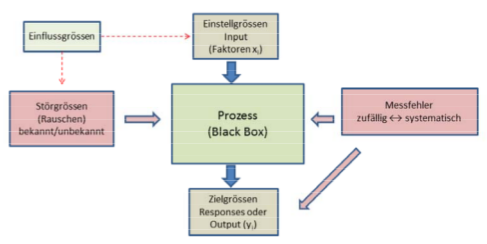
\includegraphics[scale=0.75]{img/prozessmodell.png}

\subsection{Versuchsplanung}

\begin{itemize}
	\item	Zielgrösse / Output
	\item	Einflussgrössen
	\item	Faktoren (vermutete wesentliche Einflussgrössen)
	\item	Faktorenstufen (Werte, die Faktoren in einem Experiment annehmen)
\end{itemize}

\subsection{(Mess-)Fehler}

\begin{description}
	\item[Absolute Fehler] \hfill \\
		Messfehler in einer Masseinheit
	\item[Relative Fehler] \hfill \\
		Fehler in Prozent
	\item[Zufälliger Fehler] \hfill \\
		Fehler, welcher nicht reproduzierbar auftritt (z.B. Rauschen)
	\item[Systematische Fehler] \hfill \\
		Fehler, welcher Systematisch auftritt (z.B. falsche Lineallänge, Parallax Fehler)
\end{description}

\subsubsection{Fehlerpropagation}

	Bei Multiplikation addiert sich der relative Fehler, bei Addition addiert sich der absolute Fehler.

\subsubsection{Implizite Fehlerannahme}

Bei der Impliziten Fehlerannahme geht man von $\pm$ 0.5 bis ca. 4 Einheiten der letzten angegebenen Stelle an.

Beispiel: bei $13.5 cm$ ist der Messfehler von $\pm 0.05 cm$ bis $\pm 0.4 cm$.

\section{Statistische Grundbegriffe}

\begin{description}
	\item[Mermalsträger] \hfill \\
		Der Gegenstand der statistischen Untersuchung, z.B. Utilization, Ausfallraten, Servicedauer
	\item[Grundgesamtheit] \hfill \\
		Abgrenzungsmermale, Aufteilung in Menge der Merkmalsträger, z.B. alle Messungen eines Tages, alle Maschinen einer Werkzeughalle.
	\item[Mermal] \hfill \\
		Eigenschaften eines Merkmalträgers, die bei der statistischen Untersuchung von Interesse ist.
	\item[Merkmalswert] \hfill \\
		Der Wert, welche bei Beobachtung, Befragung anfallen und statistisch ausgewertet werden.
	\item[Skala] \hfill \\
		Instrument, mit dem die Merkmalswerte bestimmt werden. Unterschieden werden: Nominalskala, Ordinalskala,  \{Intervallskala, Verhältnisskala\}(metrische Skala / Kardinalskala)
\end{description}

\subsection{Skalen}
\begin{description}
	\item[Nominalskala] \hfill \\
		Eigenschaften eines Merkmals, geordnet nach gleichen Typen. Damit lässt sich nicht gut statistisch Rechnen.
		
	\item[Ordinalskala (Rangskala)] \hfill \\
		Es wird ein Rang festgelegt für ein bestimmtes Merkmal. Dieser ist intensitätsmässig abgestuft.
		
	\item[metrische Skala] \hfill \\
		reelle Zahlen (stetig) oder ganze Zahlen (diskret) auf einer Skala angeordnet. Metrische Skalen sind immer quantitative Merkmale.
		Wird nach Intervallskala und Verhältnisskala unterschieden.
		
	\item[Intervallskala] \hfill \\
		Der Skalenwert Null ist willkürlich gewählt, kann nicht verhältnismässig ausgewertet werden.
	
	\item[Verhältnisskala] \hfill \\
		Der Skalenwert Null entspricht dem natürlichen absoluten Nullpunkt. Negative Werte sind nicht möglich, dafür kann der verhältnismässige Abstand gemessen werden.
\end{description}

\subsection{Ablauf Statistische Untersuchung}
\begin{enumerate}
	\item	Datenerhebung
		\begin{itemize}
			\item	Abgrenzung, Festlegen Untersuchungsmerkmale, Festlegung Datenumfang, erwartete Ergebnisse
			\item	Erhebungstechniken (Messungen, Zählungen, Befragungen, Beobachtungen)
			\item	Herkunft der Daten (Primärstatistik (Erhebung gezielt für Statistik), Sekundärstatistik (auf bestehender Datenbasis)
			\item Erhebungsumfang (Teil / Vollerhebung)
		\end{itemize}
	\item	Datenaufbereitung und -darstellung
		\begin{itemize}
			\item Unstrukturierte Daten aufbereiten (Strichliste, Häufigkeitstabellen, Sortierung nach Merkmalen)
		\end{itemize}
	\item	Datenanalyse
		\begin{itemize}
			\item Einfache Häufigkeitsverteilung (absolut / relativ)
			\item Komulierte Häufigkeitsverteilung, d.h. korrelieren/summieren mehrerer Häufigkeiten (dazuzählen vorangehender Häufigkeiten)
			\item Tabellarische Darstellung der Häufigkeitsbeschreibung
		\end{itemize}
	\item	Dateninterpretation
\end{enumerate}

Zu erheben sind insbesondere:
\begin{itemize}
	\item Merkmale (Faktoren)
	\item Merkmalsträgern
	\item welche Technik zur Erhebung
	\item welche Aufbereitungsverfahren
	\item welche Formen der Darstellung
	\item welche statistischen Analyseverfahren
\end{itemize}

\subsection{Lagemasse (Mittelwerte)}
\begin{description}
	\item[Modus] \hfill \\
		Merkmal, welches am häufigsten beobachtet wird.  \\
		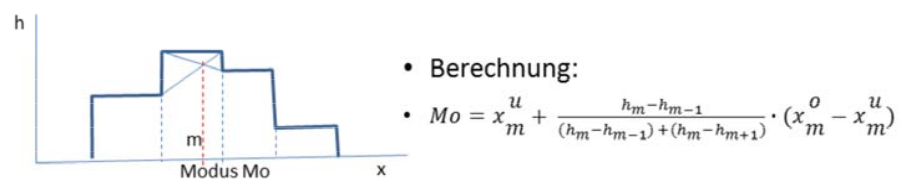
\includegraphics[scale=0.3]{img/modus.png}
	\item[Median] \hfill \\
		Wert, welcher genau in der Mitte steht bzw. den Mittelwert der beiden mittleren Werten \\
		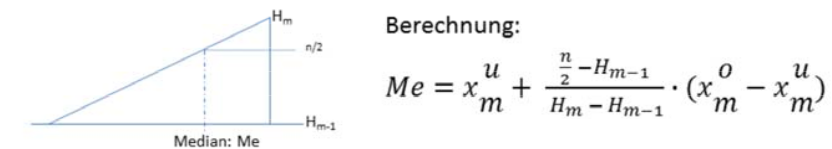
\includegraphics[scale=0.3]{img/median.png}
	\item[Quantile] \hfill \\
		Unterteilung entlang des Medians in 2 Teile. (Berechnung des Medians)
	\item[Quartil] \hfill \\
		Unterteilung in 4 Teile. (Berechnung des Medians mit $\frac{}{4}$ statt $\frac{}{2}$)
	\item[Arithmetisches Mittel] \hfill \\
		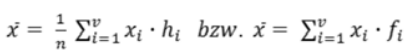
\includegraphics[scale=0.3]{img/arithmetisches_mittel.png}
	\item[Harmonisches Mittel] \hfill \\
		Berechnung: Addieren der Verhältnisse der Teilbereiche \\
		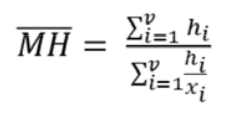
\includegraphics[scale=0.3]{img/harmonisches_mittel.png}
	\item[Geometrisches Mittel] \hfill \\
		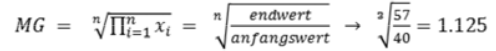
\includegraphics[scale=0.3]{img/geometrisches_mittel.png}
		
\end{description}

\subsection{Streuungsmasse}
\begin{description}
	\item[Spannweite R] \hfill \\
		R = grösster Merkmalswert - kleinster Merkmalswert. Bzw: $R = x_v^0 - x_1^u$
	\item[Zentraler Quartilsabstand] \hfill \\
		$ZQA  = Q_3 - Q_1$
	\item[Mittlere absolute Abweichung] \hfill \\
		durchschnittliche Entfernung aller Merkmalswerte vom arithmetischen Mittel: \\
		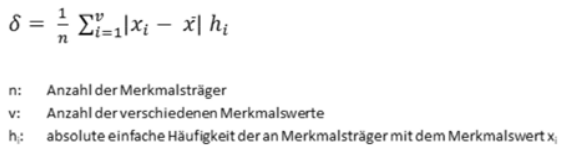
\includegraphics[scale=0.3]{img/mittlere_absolute_abweichung.png}
	\item[Varianz] \hfill \\
	Die Varianz ist die Summe der quadrierten Abweichung der Merkmalswerte vom arithmetsichen Mittel, dividiert durch die Anzahl der Merkmalsträger. \\
		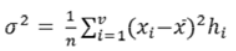
\includegraphics[scale=0.3]{img/varianz.png}
	\item[Standardabweichung] \hfill \\
		Quadratwurzel aus der Varianz
	\item[Variationskoeffizient] \hfill \\
		Quotient aus der Standardabweichung und arithmetischem Mittel, multipliziert mit 100 \\
		$VK = \frac{\sigma}{x} \cdot 100$
		
	
\end{description}

\subsection{Boxplot}

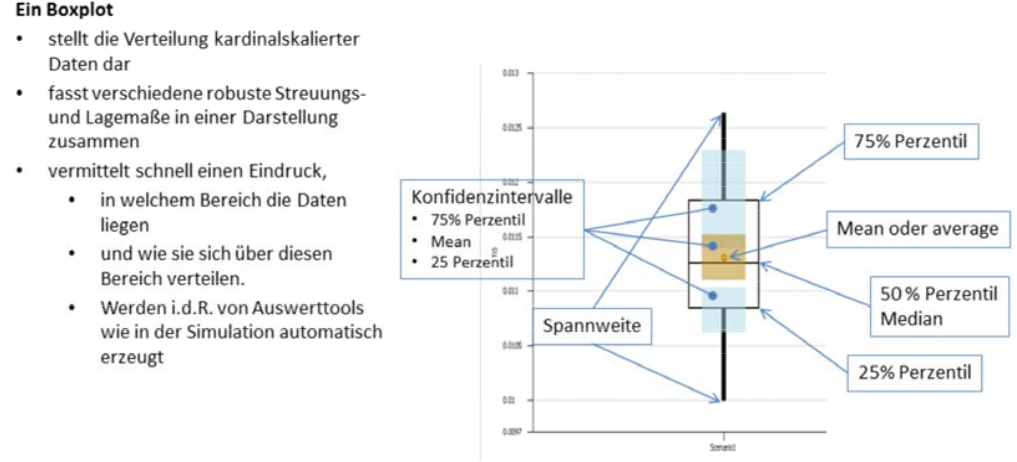
\includegraphics[scale=0.5]{img/boxplot.png}


\subsection{Grössen}

\begin{description}
	\item[$n$]		Anzahl Messungen
	\[
		n = \sum^v_{i=1}{h_j}
	\]
	\item[$v$]		Verschiedene Merkmalswerte
	\item[$h_j$] absolute Häufigkeit der Merkmalsträger mit Merkmalswert $x_i$
	\item[$h_i$] Häufigkeit eines Merkmals in einer Klasse
	\hfill \\
		% Aber wie kommt man drauf?
		\[
			\sum^{m}_{j=1}{h_j} = n
		\]
	\item[$H_j$]		Kommulierte absolute Häufigkeit
		\[
			H_j = \sum^i_{a=1}{h_a}
		\]
	\item{$x_i$}		Jeweiliger Messwert
	\item[$\acute{x}_j$] Klassenmittelwert
	\item[$\bar{x}$]	Mittelwert (Arithmetisches Mittel) des gesamten \hfill \\
		Unklassifiziert:
		\[
			\bar{x} = \frac1n \sum^v_{i=1}{x_i \cdot h_i} = \sum^v_{i=1}{x_i \cdot f_i}
		\]
		Klassifiziert:
		\[
		\bar{x} = \frac1n \sum^v_{i=1}{\acute{x}_i \cdot h_i} = \sum^v_{i=1}{\acute{x}_i \cdot f_i}
		\]
		
	\item[$\sigma$]		Standardabweichung
	\item[$\delta$]		Mittlere absolute Abweichung (Entfernung aller Merkmalswerte vom arithmetischen Mittel)
		\[
			\delta = \frac1n \sum^v_{i=1}{\left|x_i - \bar{x}\right|h_i}
		\]
	\item[$f_j$]		relative Häufigkei von $x_j$ t (mit Vorbehalt, vorherige Folie) \hfill \\
		\[
			f_j = \frac{h_j}n
		\]
	\item[$F_j$]		Kommulierte relative Häufigkeit
		\[
			F_j = \sum^i_{a=1}{f_a} = \frac{H_j}n = 1
		\]
	\item[$Q_i$]		Ein bestimmter Abschnitt $i$ in einer Unterteilung
	\item[$R$]			grösster Merkmalswert - kleinster Merkmalswert: $R = x_v^0 - x_1^u$
\end{description}

\subsection{Zeitreihe}

\subsubsection{Regressionsanalyse / Lineare Regression}

\begin{align*}
y &= a_1 + b_1 x\\
a_1 &= \bar{y} - b_1 \bar{x} \\
b_1 &= \frac{\sum^{n}_{i=1}{x_iy_i-n\bar{x}\bar{y}}}{\sum^n_{i=1}{x^2_i - n\bar{x}^2}}
\end{align*}

\subsubsection{Abhängigkeiten}
Formale Abhängigkeit: liegt eine zahlenmässig begründete Abhängigkeit zwischen den Merkmalen vor?

Sachliche Abhängigkeit: ist der Wert des einen Merkmals ursächlich (kausal) für den Wert des anderen Merkmals? (Schwierig, braucht Fachkundige)

\subsubsection{Kovarianz}
Streuung von Merkmalsträger

\section{Wahrscheinlichkeiten und Kombinatorik}

\subsection{Zufallsexperiment}

Für Experimente, deren Ergebnisse vom Zufall abhängen.

\subsection{Rechnen mit Wahrscheinlichkeiten}

\begin{align*}
P &=  \frac{\text{Gutfälle}}{\text{Mögliche Fälle}} & \text{Wahrscheinlichkeit}\\
A \cap B &= \\
A \cup B &= \\
A^c &= 1 - c & \text{Gegenereignis (komplementär)} \\
P(A|B) &= \frac{P(A \cap B)}{P(B)}
\end{align*}

\subsection{Symbole}

\begin{description}
	\item[$\Omega$] \hfill \\
		Ergebnismenge, welche sicher zutrifft. Bzw: Mögliche Zielwerte eines Experiments
	\item[$\emptyset$] \hfill \\
		Menge der unmöglichen Ereignisse.
	\item{$\sigma$-Algebra}
		Ereignisraum
	\item[Teilmengen] \hfill \\
		Ereignisse, welche Einfluss auf die Ergebnismenge $\Omega$ haben.
	\item[$\mathcal{A}$] \hfill \\
		Ganzes System, dessen Elemente Teilmengen von $\Omega$ sind.
	\item[P] \hfill \\
		Wahrscheinlichkeitsmass; Ordnet Ereignis A eine Wahrscheinlichkeit P(A) zu.
\end{description}

\subsubsection{Laplace-Experiment}

Beim Laplace-Experiment sind alle möglichen ergenisse gleich wahrscheinlich, d.h. $\mathrm{P}(A) = \frac{1}{n}$



\subsection{Kombinatorik}

\[
	\binom{n}{k} = \frac{n!}{k!(n-k)!}
\]

mit
\begin{description}
	\item[$n$] Anzahl aller Fälle
	\item[$k$] Anzahl zutreffender Fälle
\end{description}

\subsubsection{Geordnete Proben}

Permutation: Anordnung in einer Bestimmten Reihenfolge

Zahl der Permutationen ohne Wiederholungen: $n!$ bzw. mit Wiederholungen: $n^k$

\subsubsection{Ungeordnete Proben}

Für $n$ Elemente und $k$ zu vergebene Sitze.
\[
	K_k(n) = \binom{n + k -1}{k}
\]

\subsection{Rechnen}

\subsubsection{Bedingte Wahrscheinlichkeit}

Schnittmenge von zwei Vorkommnissen (Wahrscheinlichkeit für B nach Eintritt von A)

\[
	P(A|B) = \frac{P(A \cap B)}{P(B)}
\]
\[
	P(B) \cdot P(A|B) = P(A \cap B)
\]
\[
	P(B) \cdot P(A|B) = P(A) \cdot P(B|A)
\]
\[
	P(B) = \frac{P(A) \cdot P(B | A)}{P(A|B)}
\]

Stochastisch unabhängig, wenn:
\[
	P(A \cap B) = P(A) \cdot P(B)
\]


\subsection{Zufallsvariable}

Funktion, welche einen Zufälligen wert innerhalb eines bestimmten Intervalls zuweisst.

Werte, die abhängig vom Zufall sind.

Realisation einer Zufallsvariable: ''pattern''

\subsubsection{Diskrete Verteilungsdichtefunktion}

$x_i$ Eintrittswahrscheinlichkeit P eines Events $i$

Wahrscheinlichkeit eines Events $x_i$ bis $x_n$

\[
P(x_i \leq X \leq x_n) = \sum^n_{j=i}{f(x_j)}
\]

\subsubsection{Kontinuierliche Verteilungsdichtefunktion}

Fläche entspricht 1, Summe aller Wahrscheinlichkeiten

\[
P(a \leq X \leq b) = \int\limits^b_a{f(x)\mathrm{d}x}
\]

\subsubsection{Wahrscheinlichkeitsfunktion oder Verteilungs- / Summenfunktion}

\paragraph{Wahrscheinlichkeitsfunktion} Wahrscheinlichkeit von den einzelnen Teilbereichen, total $1$.

\paragraph{Verteilungs- oder Summenfunktion} Aufsummierung der Wahrscheinlichkeitsfunktion bis zum aktuellen Funktion.


\subsection{Verteilungen}
\subsubsection{Negativ exponentielle}
$f(t) = \lambda e^{-\lambda t}$

\subsubsection{Binominal}

Wenn ein gewisses Ereignis mit Wahrscheinlichkeit $p$ auftritt, ist die Wahrscheinlichkeit von bis und mit $x$ von total $n$ Fällen:

\[
	f(x) = P(X=x) = \binom{n}{x}p^x(1-p)^{n-x}
\]

\subsubsection{Poisonverteilung I}

Wie wahrscheinlich ist das Auftreten in einem Intervall?

(Diese Fragestellung erlaubt auch eine unendliche Anzahl Ereignisse.)

Wahrscheinlichkeitsfunktion:
\[
	f(x) = P(X=x) = \frac{\mu^x}{x!}e^{-\mu}
\]

Erwartungswert=Varianz
\[
	E(X) = Var(X) = \mu
\]

$\mu$ ist in diesem Zusammenhang der Durchschnitt der eingetretenen Fälle.

\subsubsection{Rechteckverteilung}

\[
	E(X) = Median = \frac{a+b}2
\]

Varianz:
\[
	Var(X) = \frac{1}{12}(b-a)^2
\]


\subsubsection{Dreieckverteilung I}

Definition:

%TODO: Picture img/dreieckverteilung

\subsubsection{Weilbull-Verteilung I}


%TODO: Picture img/weillbull

\[
	\Gamma(x) = \int^\infty_0 t^{x-1} e^{-1}
\]
\[
\Gamma(n+1) = n!
\]
für jede natürliche Zahl $n$

\subsubsection{Normalverteilung}

%TODO: Picture img/normalverteilung.png


\[
	z = \frac{x - \mu}{\sigma}
\]


\subsection{Erzeugen von Zufallszahlen}

Zufallszahlen sind nur statistisch gesehen Zufällig (wirklicher Zufall spielt keine Rolle). Es muss also reproduzierbar sein.

Also eigentlich nur Pseudo-Zufallszahlen.

\paragraph{Beispiel RNG: Linear Congruential generators:}
\[
	x_i = (a x_{i-1} + c) \mod m
\]
mit dem Ausgabewert $u_i = \frac{x_i}{m}$

\section{Theorie vs. Praxis}

\subsubsection{Stichproben}

Zwei Probleme: Genauigkeit Stichproben/Datenerhebung und Auswertung/Analyse der erhobenen Daten.

\begin{itemize}
	\item	Einfache Zufallsstichprobe
	\item	Geschichtete Stichprobe
	\item	Klumpen Stichprobe
	\item	Systematische Stichprobe
	\item	Mehrstufige Stichprobe
\end{itemize}

\section{More}

\subsubsection{Beispiel Wahrscheinlichkeit}
	
	Spiel, 1Fr. Einsatz, nach jedem Münzwurf 0.5 chance auf 1Fr.
	\\
	
	\begin{tabular}{| c c c | c | r |}
		\hline
		1 & 1 & 1 & $1/8$ & $2 \cdot 1/8$ \\
		\hline
		1 & 1 & 0 & & \\
		1 & 0 & 1 & $3/8$ & $1 \cdot 1/8$ \\
		1 & 0 & 0 &  &  \\
		\hline
		0 & 1 & 1 &  & \\
		0 & 1 & 0 & $3/8$ & $0 \cdot 3/8$ \\
		0 & 0 & 1 &  &  \\
		\hline
		0 & 0 & 0 & $1/8$ & $-1 \cdot 1/8$ \\
		\hline
		
	\end{tabular}
	\\
	
	E(x) = 0.5 Fr.

\end{document}